The Approximate Master Equation (AME) is a general mathematical equation that allows to describe binary state models in complex networks. Here, we extend the traditional mathematical framework to include aging effects, which account for the influence of the persistence time of an agent in a given state on the transition rate to a different state. When aging is considered, the Markovia assumption is no longer valid, and the AME must be modified to include non-Markovian dynamics. We derive the AME for binary-state models with aging effects, including aging and resetting events, and show how it can be reduced to the original Markovian dynamics when the rates are not dependent on the internal time. We also demonstrate how the heterogeneous mean-field approximation can be derived from the master equation. The results presented in this chapter provide a comprehensive framework for studying aging effects in binary-state models, offering a more accurate description of the dynamics of complex networks. In the following chapters of this thesis, we apply this framework to describe the aging implications in two binary-state models: the Granovetter-Watts model and the Symmetrical Threshold model.

\section{\label{sec:Introduction_binary} Introduction}

Binary-state models are a versatile tool to describe a variety of natural and social phenomena in systems formed by many interacting agents. Each agent is considered to be in one of two possible states: susceptible/infected, adopters/non-adopters, democrat/republican, etc, depending on the context of the model. The interaction among agents is determined by the underlying network and the dynamical rules of the model. There are many examples of binary-state models, including processes of opinion formation \cite{Voter-original,sood-2005,fernandez-gracia-2014,redner-2019}, disease or social contagion \cite{granovetter-1978,pastor-satorras-2015}, etc. Extended and modified versions of these models can lead to very different dynamical behaviors than in the original model. As examples, the use of multi-layer  \cite{diakonova-2014,diakonova-2016,amato-2017} or time-dependent networks \cite{vazquez-2008}, higher-order interactions \cite{de-arruda-2020, iacopini-2019, cencetti-2021}, non-linear collective phenomena \cite{castellano-2009,peralta-2018}, noise \cite{carro-2016} and non-Markovian \cite{van-mieghem-2013,starnini-2017,peralta-2020A,chen-2020} effects induce significant changes to the dynamics.

Theoretical and computational studies of stochastic binary-state models usually rely on a Markovian assumption for its dynamics. This implies that events depend only on the present state, i.e., dynamical rules are memoryless. Markovian processes exhibit exponential distributions in the upcoming events times and the number of events in a given time interval follows a Poisson distribution. However, there is strong empirical evidence against this assumption in human interactions.  For example, bursty non-Markovian dynamics with heavy-tail inter-event time distributions, reflecting temporal activity patterns,  have been reported in many studies \cite{iribarren-2009,karsai-2011,rybski-2012,zignani-2016,artime-2017,kumar-2020}. The understanding of these non-Markovian effects is in general a topic of current interest \cite{van-mieghem-2013,starnini-2017,peralta-2020C,peralta-2020A}. In particular, for the threshold models, memory effects have been included as past exposures' memory \cite{dodds-2004}, message-passing algorithms \cite{shrestha-2014}, memory distributions for retweeting algorithms \cite{gleeson-2016} and timers \cite{oh-2018}.

Aging is an important non-Markovian effect that we address in this chapter for binary-state models. We here provide a general theoretical framework to discuss aging effects building upon a general Markovian approach for binary-state models \cite{gleeson-2011,gleeson-2013}. We build an Approximate Master Equation (AME)\footnote{We use here the term  ``master equation'' for consistency with  Refs. \cite{gleeson-2011,gleeson-2013}, but the word ``master'' has a different meaning than the one used to describe an equation for the probability distribution \cite{peralta-2020B}} for any binary-state model with aging effects (including aging and resetting events). We show how the AME can be reduced to the original Markovian dynamics when the rates are not dependent on the age of the agents. We also show how the heterogeneous mean-field approximation can be derived from the master equation. The results presented in this chapter provide a solid foundation for future studies on aging effects in binary-state models, offering a more accurate description of the dynamics of complex networks. 

\section{Derivation of the Approximate Master Equation for binary-state models with aging \label{sec:Derivation of the Approximate Master Equation for binary-state models with aging}}
    
We consider  binary-state dynamics on static, undirected, connected networks assuming a locally tree-like structure and in the limit of $N \to \infty$, following closely the approach used in Ref. \cite{gleeson-2013} for binary-state dynamics in complex networks. The new ingredient is to consider the nodes with different "age" or "internal time" as different sets, what allows us to treat as Markovian the memory effects introduced by aging \cite{peralta-2020C,peralta-2020A}. We define $x^{\pm}_{k,m,j} (t)$ as the fraction of nodes that are in state $\pm 1$ and have degree $k$, $m$ infected neighbors and age $j$ at time $t$. The networks have degree distribution $p_k$ and have been generated by the configuration model \cite{molloy-1995,newman-2001}. For the models considered in this thesis, the initial condition is set such that all agents have age $j = 0$ and there is a randomly chosen fraction $x^{-}_{0}$ of nodes in state $-1$:
\begin{flalign}
    \label{initial_condition} 
    \textrm{For } j > 0 & \quad \quad    x^{+}_{k,m,j} (0) = 0 \quad \quad \quad \quad \quad \quad \quad \; \; x^{-}_{k,m,j} (0) = 0, \nonumber\\
    \textrm{For } j = 0 & \quad \quad    x^{+}_{k,m,0} (0) = (1 -  x^{-}_{0})\, B_{k,m}[x^{-}_{0}] \quad  x^{-}_{k,m,0} (0) = x^{-}_{0}\, B_{k,m}[x^{-}_{0}],
\end{flalign}
where $B_{k,m}[x^{-}_{0}]$ is the binomial distribution with $k$ attempts, $m$ successes and $x^{-}_{0}$ is the initial fraction of agents in state $-1$ (as the probability of success of the binomial). Now, we examine how $x^{+}_{k,m,j}$ changes in a time step. We consider 3 possible events:

\begin{itemize}
    \item An agent changes state from $+1$ to $-1$ and resets the internal time to $j = 0$, with probability $T^{+} (k,m,j)$.
    \item An agent remains at its state and resets its internal time to $j = 0$, with probability $R^{+} (k,m,j)$.
    \item An agent remains at its state and ages, with probability $A^{+} (k,m,j)$.
\end{itemize}

The probability to change state and to age make sense in the context of aging. The reset probability is introduced to account for ``exogenous'' aging, in which an external influence forces the node to attempt a change of state but the node remains in its current state. Moreover, notice that we assume all the probabilities to be a function of the degree $k$, the number of neighbors in state $-1$ $m$ and the time spent in the actual state (or since a reset) $j$.
\begin{figure}[ht]
    \centering
    \captionsetup{font=sf}
    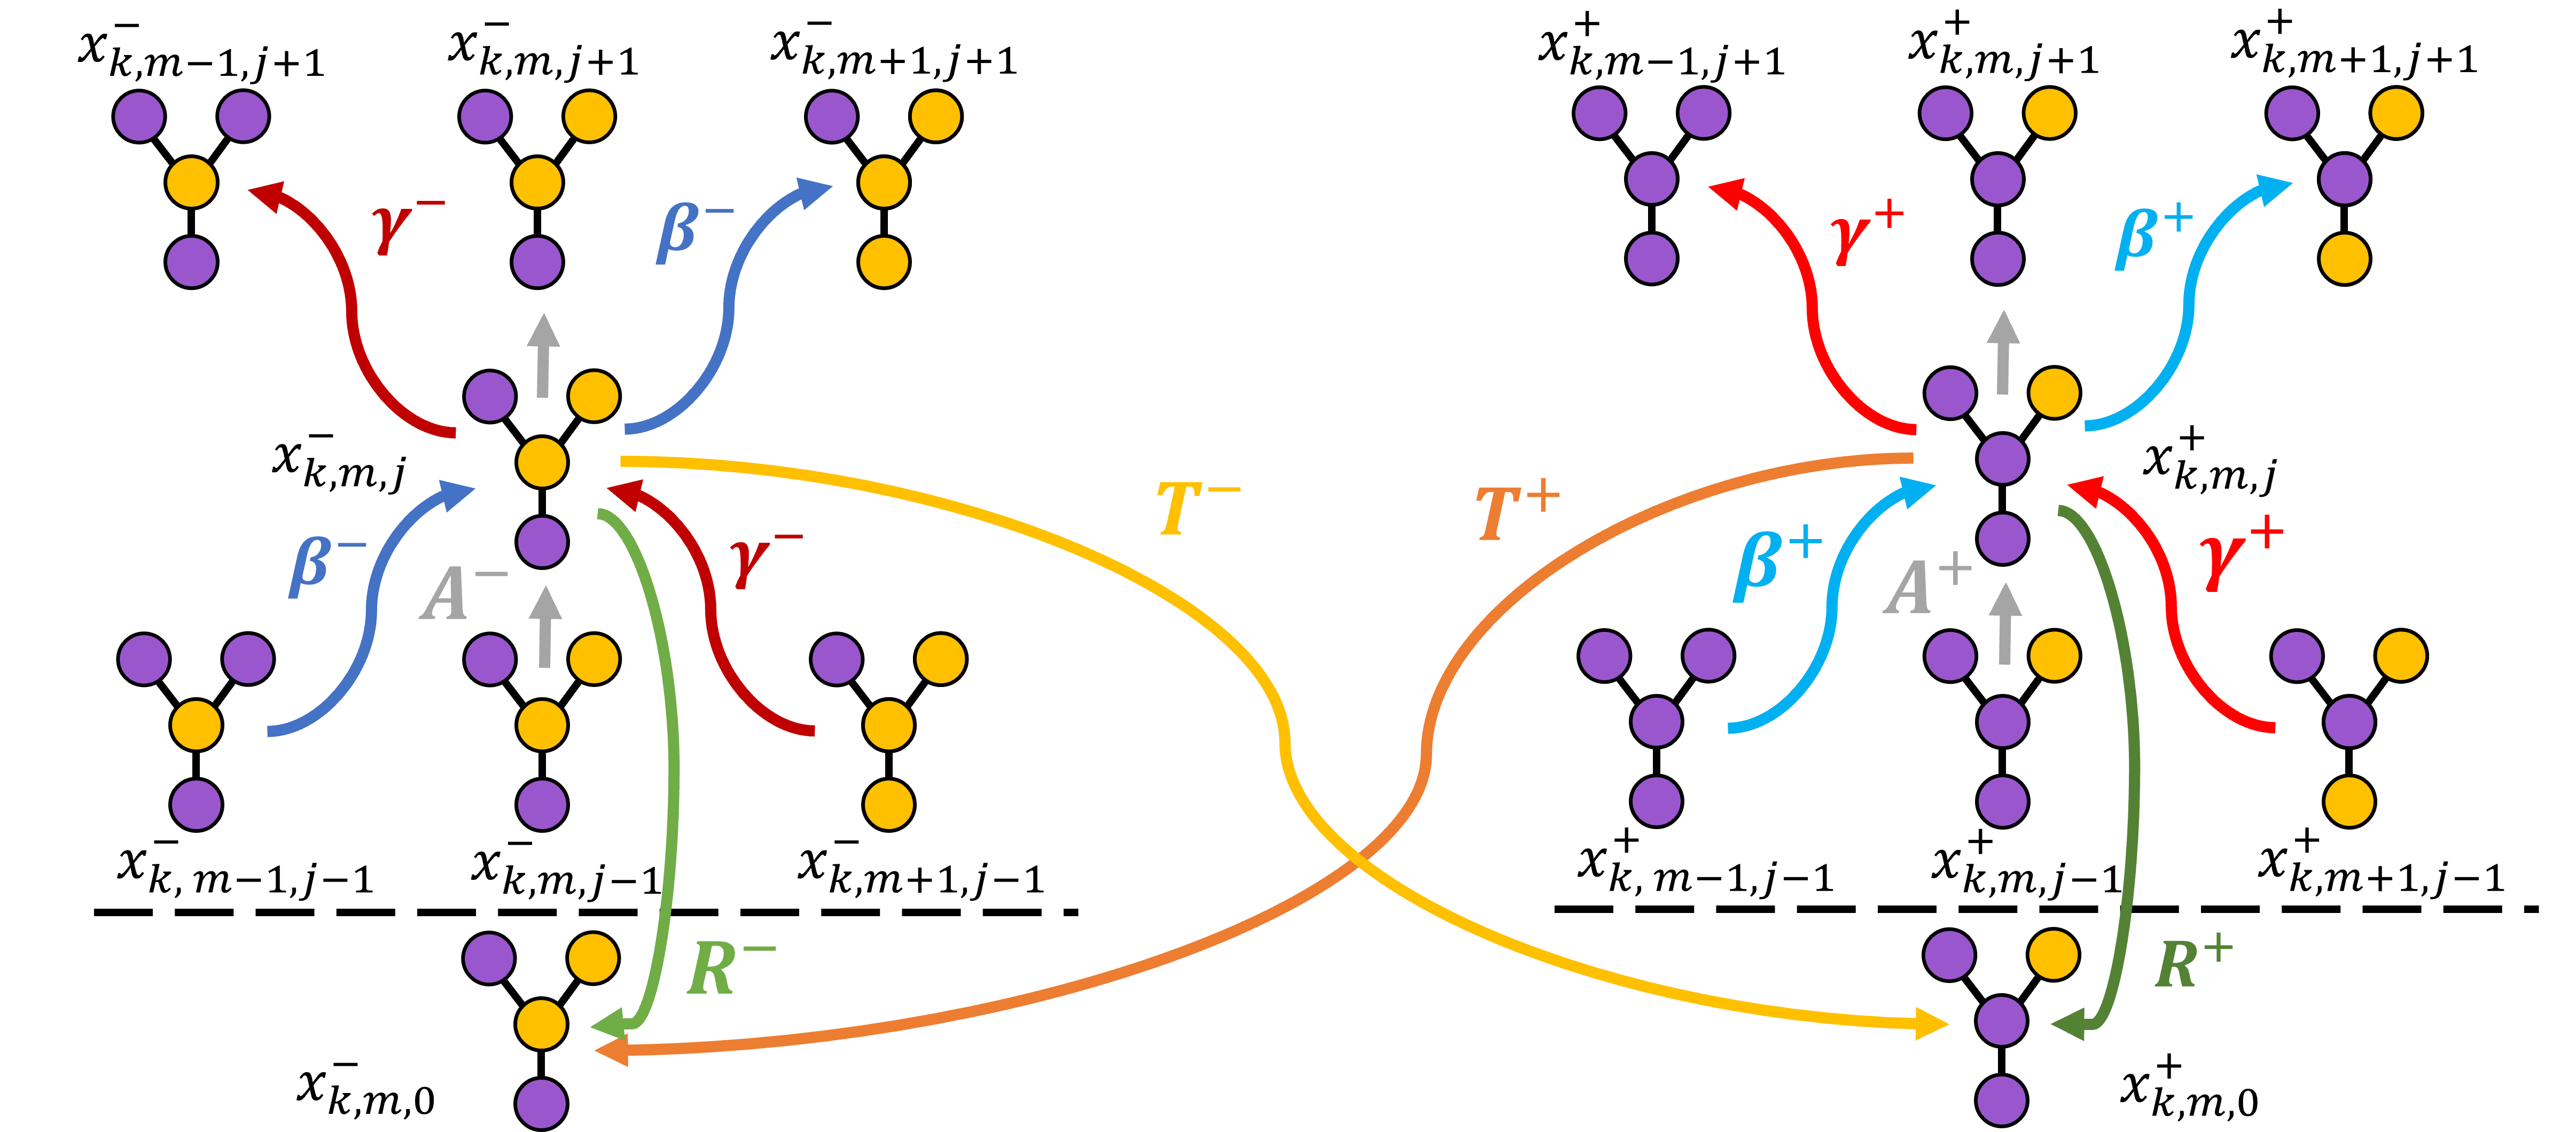
\includegraphics[width=\columnwidth]{Figs/Aging_Threshold/plot_AME_transitions.png}
    \caption[Schematic representation of the transitions to or from the set $x^{\pm}_{k,m,j}$]{\label{fig:ame_plot1} Schematic representation of the transitions to or from the set $x^{-}_{k,m,j}$ (left) and $x^{+}_{k,m,j}$ (right) ($j > 0)$. We show the central node with some neighbors ($k = 3$) for different values $m$ and $j$. Purple nodes are in state susceptible or non-adopters or $+1$, and yellow are in state infected or adopters or $-1$.}
\end{figure}
Now, taking into account this possible events, we write the possible transitions for the set $x^{+}_{k,m,j}$, for $j>0$ (see Fig. \ref{fig:ame_plot1} for a schematic representation of transitions involving $x^{+}_{k,m,j}$ and $x^{-}_{k,m,j}$):
\begin{flalign} \label{eq:pre_AME}
        x^{+}_{k,m,j} (t + dt) = & \, x^{+}_{k,m,j}(t) - T^{+} (k,m,j)\, x^{+}_{k,m,j}\, dt - R^{+} (k,m,j)\, x^{+}_{k,m,j} \, dt - A^{+} (k,m,j) \, x^{+}_{k,m,j} \, dt \nonumber \\
        & + A^{+} (k,m,j-1)\,  x^{+}_{k,m,j-1} \, dt - \omega (x^{+}_{k,m,j} \to x^{+}_{k,m+1,j+1}) \, x^{+}_{k,m,j}\, dt \\
        & - \omega (x^{+}_{k,m,j} \to x^{+}_{k,m-1,j+1})\,  x^{+}_{k,m,j} \, dt + \omega (x^{+}_{k,m+1,j-1} \to x^{+}_{k,m,j}) \, x^{+}_{k,m+1,j-1} \, dt \nonumber \\
        & + \omega (x^{+}_{k,m-1,j-1} \to x^{+}_{k,m-1,j-1}) \, x^{+}_{k,m-1,j-1}\,  dt. \nonumber
\end{flalign}
The case $j = 0$ needs to be treated differently from $j > 0$ because there is an injection of nodes into this set due to the resetting and changing state events. We write the possible transitions for the set $x^{+}_{k,m,0}$ as follows:
\begin{flalign}
        \label{eq:pre_AME_0}
        x^{+}_{k,m,0} (t + dt) = &\,  x^{+}_{k,m,0}(t) - T^{+} (k,m,0) \, x^{+}_{k,m,0} \, dt + \sum_{l = 0}^{\infty} T^{-} (k,m,l)\,  x^{-}_{k,m,l} \, dt + \sum_{l = 1}^{\infty} R^{+} (k,m,l)\,  x^{+}_{k,m,l}\,  dt   \nonumber\\
        & - T^{+} (k,m,0)\,  x^{+}_{k,m,0}\,  dt - \omega (x^{+}_{k,m,0} \to x^{+}_{k,m+1,1}) \, x^{+}_{k,m,0}\,  dt - \omega (x^{+}_{k,m,0} \to x^{+}_{k,m-1,1})\,  x^{+}_{k,m,0} \, dt.
\end{flalign}
Similar equations can be found considering transitions for $x^{-}_{k,m,j}$ and $x^{-}_{k,m,0}$. Notice that we have considered no transition increasing (or decreasing) the number of $-1$ neighbors $m$, keeping constant the age $j$. This is because the age $j$ is defined as the time spent in the current state (or since a reset). Therefore, if a node remains in its state and the number of neighbors in state $-1$ changes ($m \to m \pm 1$), the age of the node must increase ($j \to j + 1$). To determine the rate of these events, we use the same assumption as in Ref. \cite{gleeson-2013}: we assume that the number of $++$ (edges between agents in state $+1$) edges change to $+-$ edges at a time-dependent rate $\beta^{+}$. Therefore, the transition rates are:
    \begin{align} \label{rate_beta_s}
    &  \omega (x^{+}_{k,m,j} \to s_{k,m+1,j+1}) = (k - m) \, \beta^{+}, \nonumber \\
    & \omega (s_{k,m-1,j-1} \to x^{+}_{k,m,j}) = (k - m + 1)\, \beta^{+} . 
    \end{align}
To determine the rate $\beta^{+}$, we count the change of $++$ edges that change to $+-$ in a time step. This change is produced by a neighbor of a node in state $+1$ changing state from $+1$ to $-1$. Thus, we can extract this information from the transition probability $T^{+}(k,m,j)$:
\begin{equation}
        \label{beta_s}
        \beta^{+} = \frac{\sum_{j=0}^{\infty} \sum_{k=0}^{\infty} p_k \sum_{m = 0}^{k} (k - m)\, T^{+} (k,m,j) \, x^{+}_{k,m,j}}{\sum_{j=0}^{\infty} \sum_{k=0}^{\infty} p_k \sum_{m = 0}^{k} (k - m) \, x^{+}_{k,m,j}}.
\end{equation}
A similar approximation is used to determine the transition rates at which $+-$ edges change to $++$ edges. We write:
\begin{align} \label{rate_gamma_s}
    &  \omega (x^{+}_{k,m,j} \to x^{+}_{k,m-1,j+1}) = m\, \gamma^{+}, \nonumber \\
    & \omega (x^{+}_{k,m+1,j-1} \to x^{+}_{k,m,j}) = (m + 1)\, \gamma^{+} ,
\end{align}
where the rate $\gamma^{+}$ is computed using the opposite transition probability $T^{-}(k,m,j)$:
\begin{equation}
        \label{gamma_s}
        \gamma^{+} = \frac{\sum_{j=0}^{\infty} \sum_{k=0}^{\infty} p_k \sum_{m = 0}^{k} (k - m)\, T^{-} (k,m,j) \, x^{-}_{k,m,j}}{\sum_{j=0}^{\infty} \sum_{k=0}^{\infty} p_k \sum_{m = 0}^{k} (k - m)\,  x^{-}_{k,m,j}}.
\end{equation}
    
Taking the limit $dt \to 0$ of Eqs. \eqref{eq:pre_AME}-\eqref{eq:pre_AME_0}, we obtain the approximate master equation (AME) for the evolution of the different sets $x^{\pm}_{k,m,j}$ and $x^{\pm}_{k,m,0}$:
\begin{align}
\label{eq:AME}
    \frac{d x^{\pm}_{k,m,j}}{dt} = & \, - \left( T^{\pm} (k,m,j) + A^{\pm} (k,m,j) + R^{\pm} (k,m,j) \right) x^{\pm}_{k,m,j} - (k - m)\, \beta^{\pm}\,  x^{\pm}_{k,m,j} \nonumber\\
    & - m \, \gamma^{\pm}\, x^{\pm}_{k,m,j} + (k-m+1)\, \beta^{\pm} \,   x^{\pm}_{k,m-1,j-1} + (m+1)\, \gamma^{\pm} \,  x^{\pm}_{k,m+1,j-1} + A^{\pm} (k,m,j-1)\,  x^{\pm}_{k,m,j-1},  \\
    \frac{d x^{\pm}_{k,m,0}}{dt}  = & \, - \left( T^{\pm} (k,m,0) + A^{\pm} (k,m,0) + R^{\pm} (k,m,0) \right) x^{\pm}_{k,m,0} - (k - m) \, \beta^{\pm}\,  x^{\pm}_{k,m,0} - m\, \gamma^{\pm} \,  x^{\pm}_{k,m,0}\nonumber\\
    & + \sum_{l = 0}^{\infty} T^{\mp} (k,m,l)\,  x^{\mp}_{k,m,l} + \sum_{l = 0}^{\infty} R^{\pm} (k,m,l)\, x^{\pm}_{k,m,l},\nonumber
\end{align}
where $\beta^{-}$ ($\gamma^{-}$) are time-dependent rates that account for the transitions at which $-+$ ($--$) edges change to $--$ ($-+$) edges:
\begin{align}
    \beta^{-} = \frac{\sum_{j=0}^{\infty} \sum_{k=0}^{\infty} p_k \sum_{m = 0}^{k} m \, T^{+} (k,m,j) \, x^{+}_{k,m,j}}{\sum_{j=0}^{\infty} \sum_{k=0}^{\infty} p_k \sum_{m = 0}^{k} (k - m)\,  x^{-}_{k,m,j}} \quad \quad \gamma^{-} = \frac{\sum_{j=0}^{\infty} \sum_{k=0}^{\infty} p_k \sum_{m = 0}^{k} m\, T^{-} (k,m,j) \, x^{-}_{k,m,j}}{\sum_{j=0}^{\infty} \sum_{k=0}^{\infty} p_k \sum_{m = 0}^{k} m\,  x^{-}_{k,m,j}}.
\end{align}
Equations \ref{eq:AME} define a closed set of deterministic differential equations that can be solved numerically using standard computational methods for any complex network and any model aging via the transition, reset and aging probabilities (a general script in Julia is available in a GitHub repository \cite{link_git}).
    
%The binary-state model is introduced via the transition, aging and reset probabilities ($T^{\pm}, A^{\pm}, R^{\pm}$), which may depend on the degree $k$, the number $m$ of neighbors in state $-1$ and the time spent in the actual state (or since a reset) $j$. For the Granovetter-Watts model with aging (chapter \ref{ch:Aging in binary state dynamics: The Granovetter-Watts model}), dynamics are monotonic and there are no age dynamics once the agent is state $-1$ ($T^{-} (k,m,j) = A^{-} (k,m,j) = R^{-} (k,m,j) = 0$). Therefore, the equations for $x^{+}_{k,m,0}$ decouples from the equations for the variables $x^{-}_{k,m,j}$, reducing the equations to:
%\begin{align}
%\label{eq:AME_Threshold_AP}
%    \frac{d x^{+}_{k,m,j}}{dt}  = & \, - \left(T^{+}(k,m,j) + A^{+}(k,m,j) + R^{+} (k,m,j)\right) \, x^{+}_{k,m,j} - (k - m)\, \beta^{+} \,   x^{+}_{k,m,j} \nonumber\\
%    & + (k-m+1) \, \beta^{+} \,  x^{+}_{k,m-1,j-1} + A^{+} (k,m,j-1)\,  x^{+}_{k,m,j-1},  \\
%    \frac{d x^{+}_{k,m,0}}{dt}  = & \,  - \left(T^{+}(k,m,0) + A^{+}(k,m,0) + R^{+} (k,m,0)\right) \,x^{+}_{k,m,0} - (k - m)\, \beta^{+} \,  x^{+}_{k,m,0} + \sum_{l = 0}^{\infty} R^{+} (k,m,l) \, x^{+}_{k,m,l} . \nonumber
%\end{align}
%For the Symmetrical Threshold model with aging (chapter \ref{ch:Ordering dynamics in the Symmetrical Threshold model}), this monotonic approximation is no longer valid. On the other hand, for this model we do not consider age resetting ($R^{\pm} (k,m,j) = 0$) since aging is "endogenous". Therefore, the equations to solve are:
%\begin{align}
%\label{eq:AME_Threshold_SP}
%    \frac{d x^{\pm}_{k,m,j}}{dt}  = & \, - \left( T^{\pm} (k,m,j) + A^{\pm} (k,m,j) + R^{\pm} (k,m,j) \right) \, x^{\pm}_{k,m,j} - (k - m)\, \beta^{\pm} \,  x^{\pm}_{k,m,j} - m\, \gamma^{\pm} \,  x^{\pm}_{k,m,j} \nonumber\\
%    & + (k-m+1)\, \beta^{\pm} \,  x^{\pm}_{k,m-1,j-1} \, + (m+1)\, \gamma^{\pm} \,  x^{\pm}_{k,m+1,j-1} + A^{\pm} (k,m,j-1)\,  x^{\pm}_{k,m,j-1},\\
%    \frac{d x^{\pm}_{k,m,0}}{dt}  = & \, - \left( T^{\pm} (k,m,0) + A^{\pm} (k,m,0) + R^{\pm} (k,m,0) \right) \, x^{\pm}_{k,m,0} - (k - m)\, \beta^{\pm} \,  x^{\pm}_{k,m,0} - m\, \gamma^{\pm} \,  x^{\pm}_{k,m,0}\nonumber\\
%    &+ \sum_{l = 0}^{\infty} T^{\mp} (k,m,l) \,  x^{\mp}_{k,m,l}.\nonumber 
%\end{align}

\section{\label{sec:Reduction to Markovian dynamics}  Reduction to Markovian dynamics}

When there are neither resetting nor aging events ($R^{\pm} (k,m,j) = A^{\pm} (k,m,j) = 0$) and the transition probabilities do not depend on the internal time $j$, $T^{\pm} (k,m,j) = T^{\pm} (k,m)$, our dynamics are Markovian. In this case, if we are not interested in the solutions $x^{\pm}_{k,m,j} (t)$, Eq. \ref{eq:AME} can be reduced by summing variable $j$. We define $x^{\pm}_{k,m} = \sum_{j} x^{\pm}_{k,m,j}$ as the fraction of nodes that are in state $\pm 1$ and have degree $k$ and $m$ infected neighbors. The equations for the variables $x^{\pm}_{k,m}$ are:

\begin{align}
\label{eq:AME_noage}
    \frac{d x^{\pm}_{k,m}}{dt} = \frac{d x^{\pm}_{k,m,0}}{dt} + \sum _{j=1}^{\infty} \frac{d x^{\pm}_{k,m,j}}{dt}  = & \, - T^{\pm} (k,m) \, x^{\pm}_{k,m} + T^{\mp}(k,m) \, x^{\mp}_{k,m} - (k - m)\, \beta^{\pm} \,  x^{\pm}_{k,m} - m\, \gamma^{\pm} \,  x^{\pm}_{k,m} \nonumber\\
    & + (k-m+1)\, \beta^{\pm} \,  x^{\pm}_{k,m-1} \, + (m+1)\, \gamma^{\pm} \,  x^{\pm}_{k,m+1},
\end{align}
where the rates $\beta^{\pm}$ and $\gamma^{\pm}$ are redefined as follows:
\begin{align}
    & \beta^{+} = \frac{\sum_{k=0}^{\infty} p_k \sum_{m = 0}^{k} (k - m)\, T^{+} (k,m) \, x^{+}_{k,m}}{\sum_{k=0}^{\infty} p_k \sum_{m = 0}^{k} (k - m)\,  x^{-}_{k,m}}, \quad \quad \gamma^{+} = \frac{\sum_{k=0}^{\infty} p_k \sum_{m = 0}^{k} (k-m)\, T^{+} (k,m) \, x^{+}_{k,m}}{\sum_{k=0}^{\infty} p_k \sum_{m = 0}^{k} m\,  x^{+}_{k,m}}, \nonumber\\
    & \beta^{-} = \frac{\sum_{k=0}^{\infty} p_k \sum_{m = 0}^{k} m \, T^{+} (k,m) \, x^{+}_{k,m}}{\sum_{k=0}^{\infty} p_k \sum_{m = 0}^{k} (k - m)\,  x^{-}_{k,m}}, \quad \quad \quad \quad \; \gamma^{-} = \frac{\sum_{k=0}^{\infty} p_k \sum_{m = 0}^{k} m\, T^{-} (k,m) \, x^{-}_{k,m}}{\sum_{k=0}^{\infty} p_k \sum_{m = 0}^{k} m\,  x^{-}_{k,m}}.
\end{align}
Notice that this reduction is not an approximation and there is no loss of accuracy. The reduction to Markovian dynamics is a consequence of the chosen model. Eq. \ref{eq:AME_noage} correspond to the equations derived by J.P. Gleeson \cite{gleeson-2013} for Markovian binary-state dynamics in complex networks. This is a set of $(k_{\rm max}+1)(k_{\rm max}+1)$ differential equations that can be solved numerically using standard computational methods for any complex network and any model via the transition probabilities $T^{\pm} (k,m)$.

%For the Symmetrical threshold model (chapter \ref{ch:Ordering dynamics in the Symmetrical Threshold model}), the dynamics are Markovian since the transition rates (if we forget about the age dynamics) are:

%\begin{align}
%    T^{+} (k,m) = \theta \left(\frac{m}{k} - T \right) \quad \quad T^{-} (k,m) = \theta \left( \frac{k-m}{k} - T \right).
%\end{align}

\section{\label{sec:Heterogeneous mean-field approximation}  Heterogeneous mean-field approximation (HMF)}

Moreover, from Eqs. \eqref{eq:AME_noage}, we can perform a heterogeneous mean-field approximation (HMF) to reduce our system to $k_{\rm max}+1$ differential equations \cite{gleeson-2013}. This appoximation assumes a solution $x^{\pm}_{k,m} = x_{k}^{\pm} B_{k,m} [\omega]$, where $\omega = \langle k x^{-}_{k} \rangle / \langle k \rangle$ is the probability that one end of a randomly chosen edge is in state $-1$. Using this ansatz, the AME can be reduced to the following set of equations:

\begin{eqnarray}
    \frac{d}{d t} x^{-}_{k}= &- x^{-}_{k} \sum_{m=0}^{k} T^{-}_{k, m} B_{k, m}[\omega] +\left(1-x^{-}_{k}\right) \sum_{m=0}^{k} T^{+}_{k, m} B_{k, m}[\omega],
    \label{eq:HMF}
\end{eqnarray}
This system of $(k_{\rm max}+1)$ differential equations, coupled via $\omega$, cannot be solved analytically in general. However, it can be solved numerically using standard computational methods.

%In particular, for the Symmetrical Threshold model, HMF predicts a mixed-ordered transition line that qualitatively captures the critical line dependence but quantitatively differs from the numerical simulations (see the red dashed line in Figs. \ref{ER_REG_PD}a and \ref{ER_REG_PD}b and the dotted colored lines in Fig. \ref{ER_REG_PD}c). Moreover, this approximation does not predict a frozen phase in any of the networks considered. Instead, for high values of $T$, the integrated stationary solutions are always $m_f = \pm 1$, regardless of $m_0$. From this analysis, we conclude that we need sophisticated methods beyond an HMF description to describe the Symmetrical Threshold model's phase diagram (in a random sparse network).

\section{\label{sec:Summary} Summary and discussion}

This chapter has expanded traditional binary-state models to include the effects of aging, providing a deeper insight into the dynamic behavior of complex networks. The mathematical framework developed here lays the groundwork for future studies to explore various aspects of aging in other dynamic systems, potentially leading to more accurate predictions and control strategies in both natural and engineered networks. The results presented in this chapter are a significant step forward in understanding the role of aging in binary-state dynamics, and we hope that they will inspire further research in this area.

Further work in this area could include the inclusion of other non-Markovian effects, such as memory kernels \cite{saeedian2017memory} or extended to 3-state dynamics, which could be useful to understand the phase diagram of the Sakoda-Schelling model with aging, described in previous chapter. Moreover, the AME was improved in Ref. \cite{peralta-2020C} to include finite-size and stochastic effects in binary-state models, which could be extended to include aging effects. Finally, the framework developed in this chapter could be useful to describe aging dynamics in threshold models, since these models need for a mathematical framework that needs to go beyond mean-field approximations to capture the dynamics of the system \cite{gleeson-2007}.